\documentclass[a4paper,12pt]{article}

\usepackage[utf8]{inputenc}
\usepackage[russian]{babel}
\usepackage[T2A]{fontenc}
\usepackage{amsmath,amssymb}
\usepackage{graphicx}
\usepackage{booktabs}
\usepackage{longtable}
\usepackage{caption}
\usepackage{geometry}
\geometry{margin=2cm}
\graphicspath{{figs/}} % предполагается, что все графики лежат в analysis_py/figs

\begin{document}

\begin{center}
    \Large
    Исследование алгоритма имитации отжига\\
    для задачи многопроцессорного расписания:\\
    сравнение последовательной и параллельной реализаций
\end{center}

\vspace{1em}

\noindent
Цель работы: реализовать и исследовать метод имитации отжига для постановки \textbf{$P||\sum C_j$} (минимизация суммы времён завершения всех работ на $M$ однородных процессорах) и сравнить поведение последовательной и параллельной версий алгоритма по скорости и качеству решения на задачах крупного размера.


% ============================================================
\section{Постановка задачи}

Рассматривается множество $N$ независимых работ с длительностями $p_j > 0$, $j=1,\dots,N$, и $M$ идентичных параллельных исполнителей (процессоров). Необходимо распределить работы по процессорам и упорядочить их на каждом процессоре.

Пусть $C_j$ --- время завершения работы $j$ в построенном расписании. Целевая функция:
\[
    K_2 = \sum_{j=1}^{N} C_j.
\]
Задача $P||\sum C_j$ является NP-трудной; точная оптимизация при больших $N$ не рассматривается, используются эвристики.

Также измеряются вспомогательные метрики:
\begin{itemize}
    \item \textbf{makespan} (максимальное время завершения среди всех работ, то есть длина расписания по самому загруженному процессору);
    \item \textbf{суммарная стоимость $K_2$} (основная метрика качества);
    \item \textbf{время работы алгоритма} (в миллисекундах стендового времени).
\end{itemize}

Далее под \emph{качеством} будем понимать именно $K_2 = \sum C_j$: чем меньше, тем лучше.

% ============================================================
\section{Структура программы и алгоритм}

В проекте реализованы три ключевых исполняемых файла (CMake $\geq$ 3.20):
\begin{itemize}
    \item \texttt{sa\_seq} --- последовательная реализация имитации отжига;
    \item \texttt{sa\_par} --- параллельная (многопоточная) версия;
    \item \texttt{research} --- утилита для проведения серий экспериментов, агрегации результатов и экспорта их в \texttt{.csv}.
\end{itemize}

Архитектура кода разделена на заголовки (\texttt{include/}) и реализации (\texttt{src/}):

\begin{itemize}
    \item модуль расписания: структура \texttt{Schedule}, которая хранит очереди работ по процессорам и позволяет вычислить стоимость расписания ($\sum C_j$) и makespan;
    \item модуль оценки: функции вычисления $K_2$ для данного расписания;
    \item модуль соседства (neighborhood): генератор локальных перестановок расписания (перенос работы между процессорами, обмен двух работ и т.\,п.);
    \item модуль имитации отжига:
    \begin{itemize}
        \item \texttt{SequentialAnnealer}: одна цепочка имитации отжига;
        \item \texttt{ParallelAnnealerManager}: менеджер, который запускает несколько независимых цепочек отжига в разных потоках и периодически выбирает лучшее найденное расписание.
    \end{itemize}
    \item служебные модули: генератор случайных чисел (с фиксируемым seed), таймер, парсер аргументов командной строки, профили охлаждения температуры.
\end{itemize}

\subsection*{Имитация отжига (SA)}

Последовательная цепочка SA поддерживает текущее расписание $S$ и его стоимость $f(S)=\sum C_j$. На каждом шаге генерируется соседнее решение $S'$ путём локальной модификации $S$. Пусть $\Delta = f(S')-f(S)$.
\begin{itemize}
    \item Если $\Delta \le 0$, то $S'$ принимается всегда.
    \item Если $\Delta > 0$, то $S'$ принимается с вероятностью
    \[
        P = \exp\!\left(-\frac{\Delta}{T}\right),
    \]
    где $T$ --- текущая температура.
\end{itemize}
Температура $T$ убывает по заданному закону охлаждения (геометрическому, линейному или Коши-подобному). Таким образом, в начале поиск «разрешает ухудшения» и исследует пространство, а затем постепенно «замерзает» и становится жадным.

Критерии остановки цепочки: лимит по числу итераций и лимит по числу шагов без улучшения глобально лучшего найденного решения.

\subsection*{Параллельная версия}

Параллельная версия не пытается распараллелить \emph{одну} цепочку SA. Вместо этого менеджер запускает несколько \emph{независимых} цепочек SA (по числу потоков), каждая из которых ищет улучшения. По завершении раунда потоков лучшее найденное расписание записывается в общий «глобальный рекорд». Далее от этого глобально лучшего решения стартует следующий раунд.

Важно: параллельная версия делает существенно больше совокупной работы (несколько цепочек, возможны несколько «волн» запуска при отсутствии улучшения). Значит, сырое время работы параллельной версии не является «ускорением» той же самой нагрузки; это скорее «более интенсивный поиск за большее время».

% ============================================================
\section{Методика эксперимента}

Эксперименты проводились автоматизированно программой \texttt{research}, которая:
\begin{itemize}
    \item генерирует случайные экземпляры задачи (фиксируется число процессоров $M=4$, далее варьируется число работ $N$ и их длительности);
    \item запускает либо последовательную версию (\texttt{mode=seq}, \texttt{threads=0}), либо многопоточную версию (\texttt{mode=par}, \texttt{threads} $\in \{2,4,6,12\}$);
    \item повторяет запуск несколько раз (\texttt{runs} = 2--5 в зависимости от размера задачи), усредняет время исполнения (\texttt{avg\_time\_ms}) и запоминает лучшую найденную стоимость (\texttt{best\_cost});
    \item записывает результаты в формат \texttt{CSV}.
\end{itemize}

Мы использовали:
\begin{itemize}
    \item Набор «основных» инстансов: $N \in \{100, 500, 1000, 10000\}$, $M=4$, \texttt{threads} $\in \{0,2,4,6,12\}$. Эти данные далее визуализируются на линейных и столбчатых графиках.
    \item Масштабное сканирование (тепловые карты): $N$ от $100$ до $4850$ с шагом $250$, \texttt{threads} от $1$ до $12$. Это даёт матрицу $20 \times 12 = 240$ измерений для времени и качества.
\end{itemize}

Замеры проводились на машине с 12 аппаратными потоками исполнения. Это значит, что \texttt{threads=12} примерно соответствует полной загрузке CPU.

Далее приводятся результаты. Для краткости будем использовать следующие определения:
\begin{itemize}
    \item \textbf{Время} --- \texttt{avg\_time\_ms}, среднее стендовое время работы алгоритма (мс).
    \item \textbf{Стоимость} --- \texttt{best\_cost} $= \sum C_j$, чем меньше, тем лучше.
    \item \textbf{Относительное качество} \(\texttt{rel\_cost\_pct}\): для фиксированного $N$ считаем 100\% как \emph{лучшее} найденное среди всех алгоритмов значение $K_2$; остальные алгоритмы выражаем как долю от лучшего. Например, 100.2\% означает решение хуже на 0.2\%.
    \item \textbf{Ускорение по времени} (\texttt{speed\_gain\%}): \(\displaystyle 100 \cdot T_{\text{seq}} / T_{\text{par}}\). Значение $>100\%$ означало бы, что параллельная версия быстрее последовательной. Значение $<100\%$ означает, что параллельная версия работает медленнее.
\end{itemize}

\bigskip
Исходные таблицы данных взяты из файлов \texttt{.csv}, предоставленных по итогам прогона \texttt{research}.

% ============================================================
\section{Результаты и анализ}

\subsection{Сравнение времени исполнения и качества \\(фиксированное $M=4$, $N \in \{100,500,1000,10000\}$)}

На рис.~\ref{fig:line_time} показано среднее время исполнения \texttt{avg\_time\_ms} в логарифмическом масштабе по оси $Y$ (график \texttt{line\_time\_cmp.png}). По оси $X$ откладываются только реально измеренные значения $N$, но точки расположены равномерно, чтобы избежать «сжатия» крупных $N$.

\begin{figure}[h!]
    \centering
    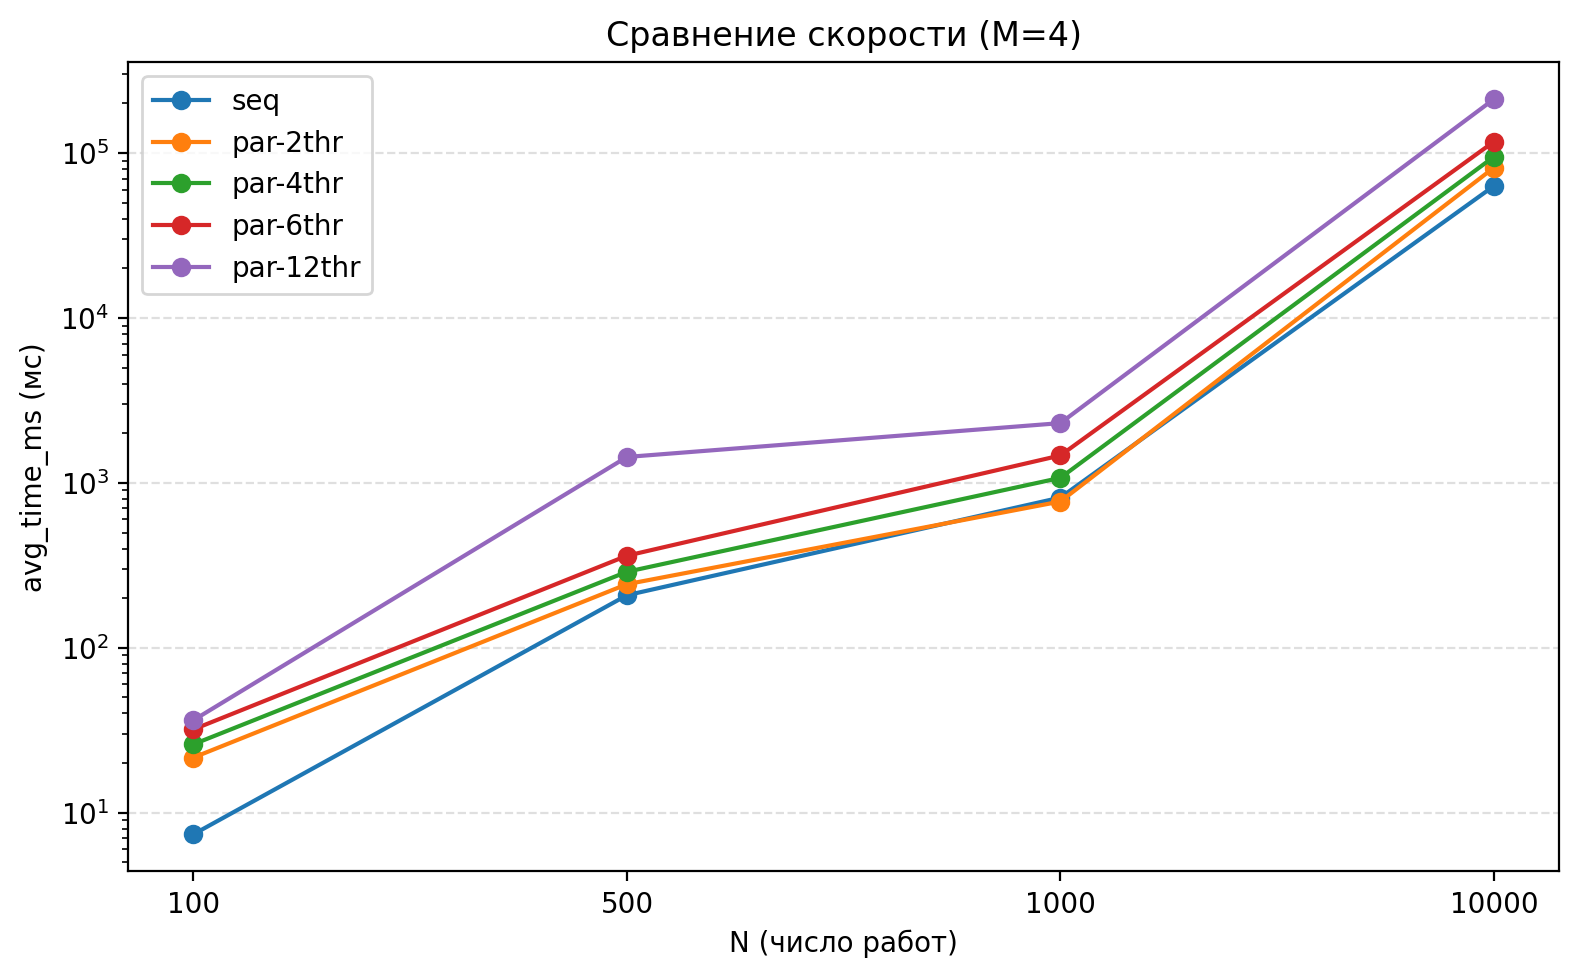
\includegraphics[width=0.8\textwidth]{line_time_cmp.png}
    \caption{Среднее время работы алгоритмов в зависимости от размера задачи $N$.
    На графике присутствуют последовательный вариант (\texttt{seq}, threads=0) и параллельные варианты с разным числом потоков.
    Ось $Y$ логарифмическая.}
    \label{fig:line_time}
\end{figure}

Наблюдения:
\begin{itemize}
    \item Последовательная версия (\texttt{threads=0}) стабильно самая быстрая.
    \item Увеличение числа потоков \emph{не} приводит к уменьшению стендового времени. Напротив, при \texttt{threads=12} время может быть на порядок больше.
    \item Это ожидаемо для \emph{нашей} параллельной схемы: мы запускаем несколько независимых цепочек отжига, фактически выполняя \emph{более объёмную} работу поиска. Мы не делим одну и ту же работу на потоки, мы делаем много независимых попыток улучшиться.
\end{itemize}

Для количественной иллюстрации приведём агрегированную таблицу (см. табл.~\ref{tab:main-results}). В таблице:
\begin{itemize}
    \item \texttt{time\_ms} --- среднее время в мс;
    \item \texttt{cost} --- лучшая найденная стоимость $\sum C_j$ для данной конфигурации;
    \item \texttt{speed\_gain\%} --- ускорение по времени относительно последовательной версии при том же $N$ (100\% = такая же скорость, $<100\%$ --- медленнее);
    \item \texttt{rel\_cost\%} --- качество в процентах относительно лучшего найденного для данного $N$ (100\% = лучшее среди всех алгоритмов; чем больше 100, тем хуже).
\end{itemize}

\begin{table}[h!]
\centering
\caption{Сводные результаты по времени и качеству для $M=4$, $N\in\{100,500,1000,10000\}$, threads$\in\{0,2,4,6,12\}$.}
\label{tab:main-results}
\begin{tabular}{r r r r r r}
\toprule
$N$ & Потоки & time\_ms & cost & speed\_gain\% & rel\_cost\% \\
\midrule
100 & 0  & 7.4     & 24276      & 100.0 & 100.074 \\
100 & 2  & 21.6    & 24312      & 34.3  & 100.223 \\
100 & 4  & 26.0    & 24285      & 28.5  & 100.111 \\
100 & 6  & 32.0    & 24258      & 23.1  & 100.000 \\
100 & 12 & 36.4    & 24267      & 20.3  & 100.037 \\
\midrule
500 & 0  & 208.3   & 531497     & 100.0 & 100.121 \\
500 & 2  & 243.0   & 531218     & 85.7  & 100.068 \\
500 & 4  & 289.0   & 531177     & 72.1  & 100.060 \\
500 & 6  & 361.7   & 530904     & 57.6  & 100.009 \\
500 & 12 & 1436.3  & 530856     & 14.5  & 100.000 \\
\midrule
1000 & 0   & 814.5   & 2135053    & 100.0 & 100.029 \\
1000 & 2   & 771.0   & 2137314    & 105.6 & 100.135 \\
1000 & 4   & 1072.5  & 2134951    & 75.9  & 100.024 \\
1000 & 6   & 1466.5  & 2134780    & 55.5  & 100.016 \\
1000 & 12  & 2304.0  & 2134438    & 35.4  & 100.000 \\
\midrule
10000 & 0   & 63145.0  & 213451049   & 100.0 & 100.215 \\
10000 & 2   & 81565.0  & 213072512   & 77.4  & 100.037 \\
10000 & 4   & 94987.0  & 213102178   & 66.5  & 100.051 \\
10000 & 6   & 117234.0 & 213031505   & 53.9  & 100.018 \\
10000 & 12  & 212264.0 & 212993675   & 29.7  & 100.000 \\
\bottomrule
\end{tabular}
\end{table}

Основные выводы из табл.~\ref{tab:main-results}:
\begin{itemize}
    \item \textbf{По времени.} Для больших $N$ последовательный запуск остаётся быстрее (100\% --- базовая скорость). Параллельные варианты оказываются медленнее (например, при $N=10000$ и 12 потоках мы видим лишь $\approx 29.7\%$ от скорости последовательной версии), что естественно: параллельный режим делает существенно больше итераций поиска и поэтому объективно дольше работает.
    \item \textbf{По качеству.} Разница в качестве крайне мала в относительных процентах. Для $N=10000$ лучшее найденное решение достигается при 12 потоках, и качество последовательного алгоритма хуже примерно на $0.215\%$. Даже при меньших $N$ отрыв между худшим и лучшим вариантом в пределах $0.1\%$--$0.2\%$. Для реальных значений $K_2$, которые порядка $2\cdot 10^8$ при $N=10000$, это всё же заметная экономия в абсолютных единицах.
\end{itemize}

Рис.~\ref{fig:bar_rel_cost} визуализирует относительное качество (\texttt{bar\_cost\_rel\_cmp.png}) в виде сгруппированной гистограммы: по оси $X$ --- $N$, для каждого $N$ показаны все конфигурации по числу потоков. Ось $Y$ начинается с $100\%$, то есть 100\% означает лучшее решение среди всех алгоритмов при данном $N$. Значения чуть выше 100\% означают, что решение хуже на доли процента.

\begin{figure}[h!]
    \centering
    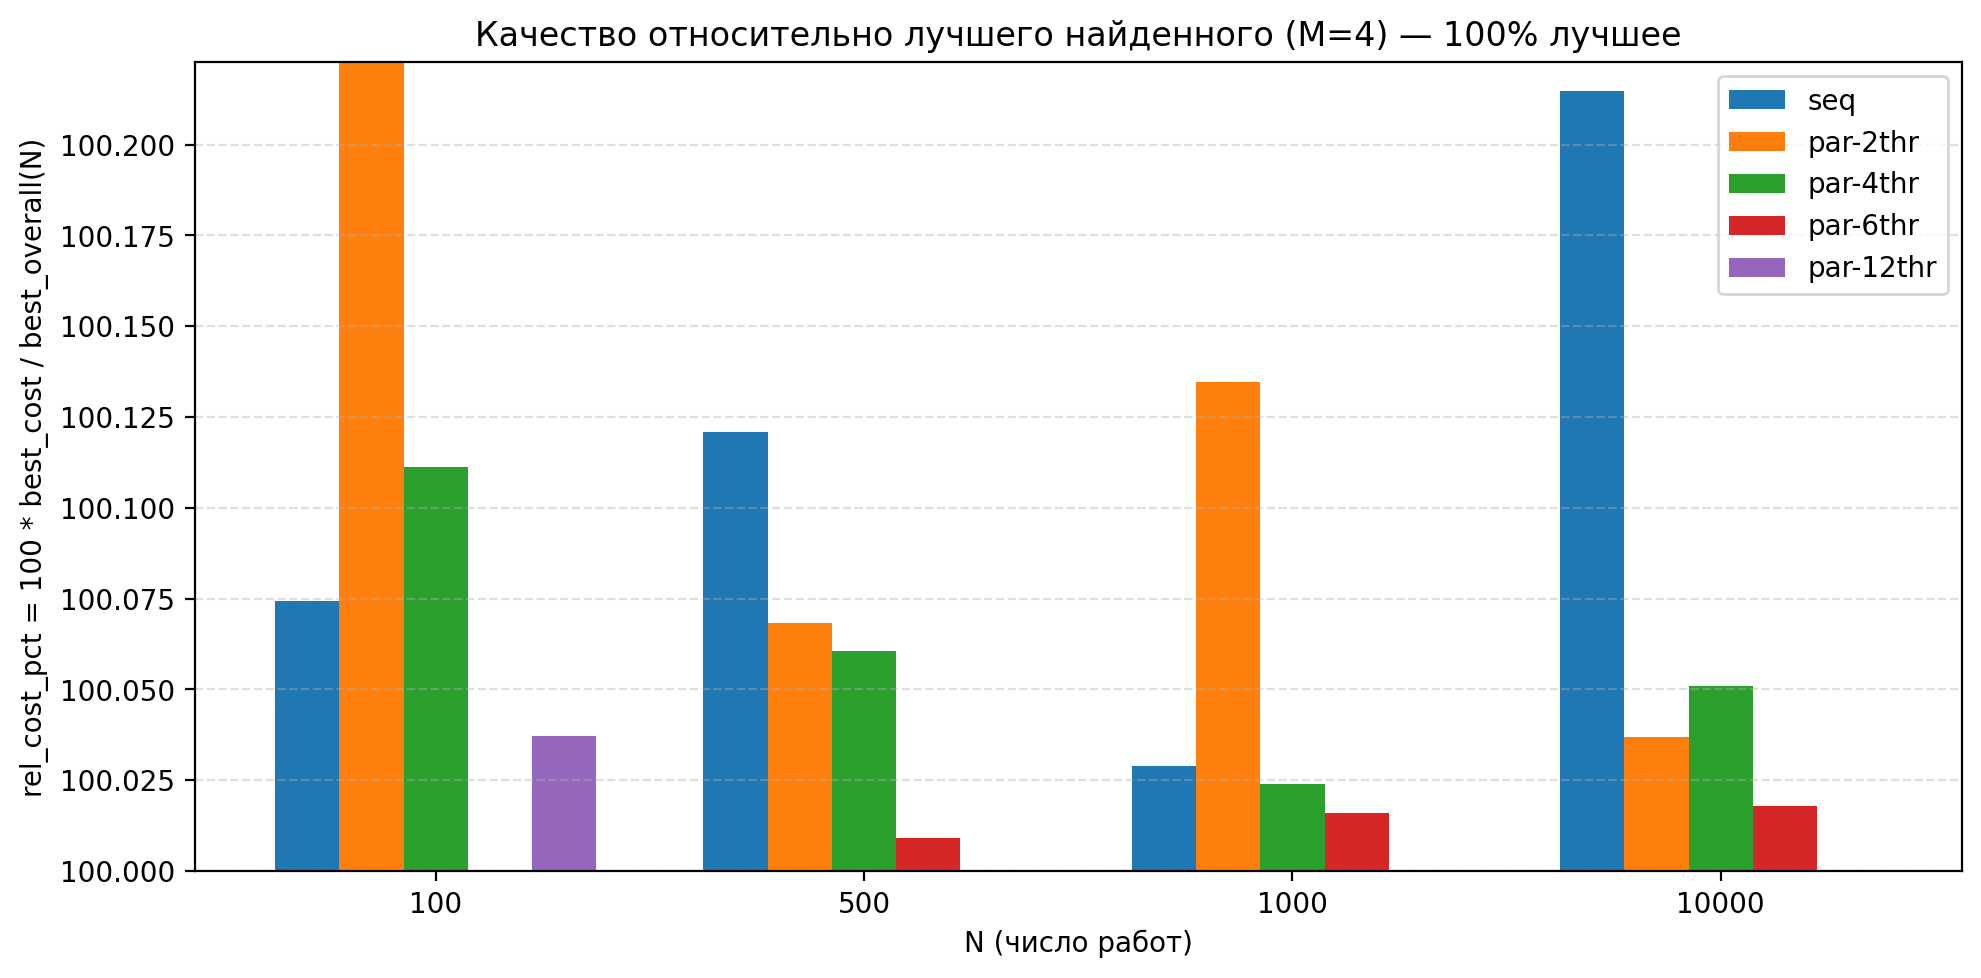
\includegraphics[width=0.8\textwidth]{bar_cost_rel_cmp.png}
    \caption{Сравнение качества (нормировано к лучшему найденному при данном $N$, 100\% = лучший найденный $K_2$). Видно, что все варианты дают решения, отличающиеся менее чем на 0.3\%.}
    \label{fig:bar_rel_cost}
\end{figure}

Также строились графики:
\begin{itemize}
    \item \texttt{line\_cost\_cmp.png} --- абсолютные значения $\sum C_j$;
    \item \texttt{line\_cost\_excess\_cmp.png} --- \emph{отрыв} от лучшего найденного решения при фиксированном $N$.
\end{itemize}
На \texttt{line\_cost\_excess\_cmp.png} ось $Y$ построена в специальной квазилогарифмической шкале: значение $0$ (лучшее решение среди всех вариантов потоков) идёт отдельной отметкой, далее идут уровни $1$, $10$, $10^2$, $10^3$, \dots\ с равными промежутками. Это позволяет визуально различать очень малые различия качества (разница в единицы и десятки по $K_2$ на фоне миллионов и сотен миллионов).

\subsection{Относительный выигрыш по времени и по качеству}

На рис.~\ref{fig:speed_quality_gain} приведены гистограммы:
\begin{itemize}
    \item \texttt{bar\_speed\_gain.png} --- \emph{ускорение} по времени выполнения относительно последовательного алгоритма (100\% = такая же скорость, больше 100\% означало бы ускорение);
    \item \texttt{bar\_quality\_gain.png} --- относительное улучшение качества по сравнению с последовательным алгоритмом (\(100 \cdot C_{\text{seq}} / C_{\text{par}}\)). Здесь шкала по $Y$ начинается от 100\% и тянется вверх, чтобы сделать различия видимыми.
\end{itemize}

\begin{figure}[h!]
    \centering
    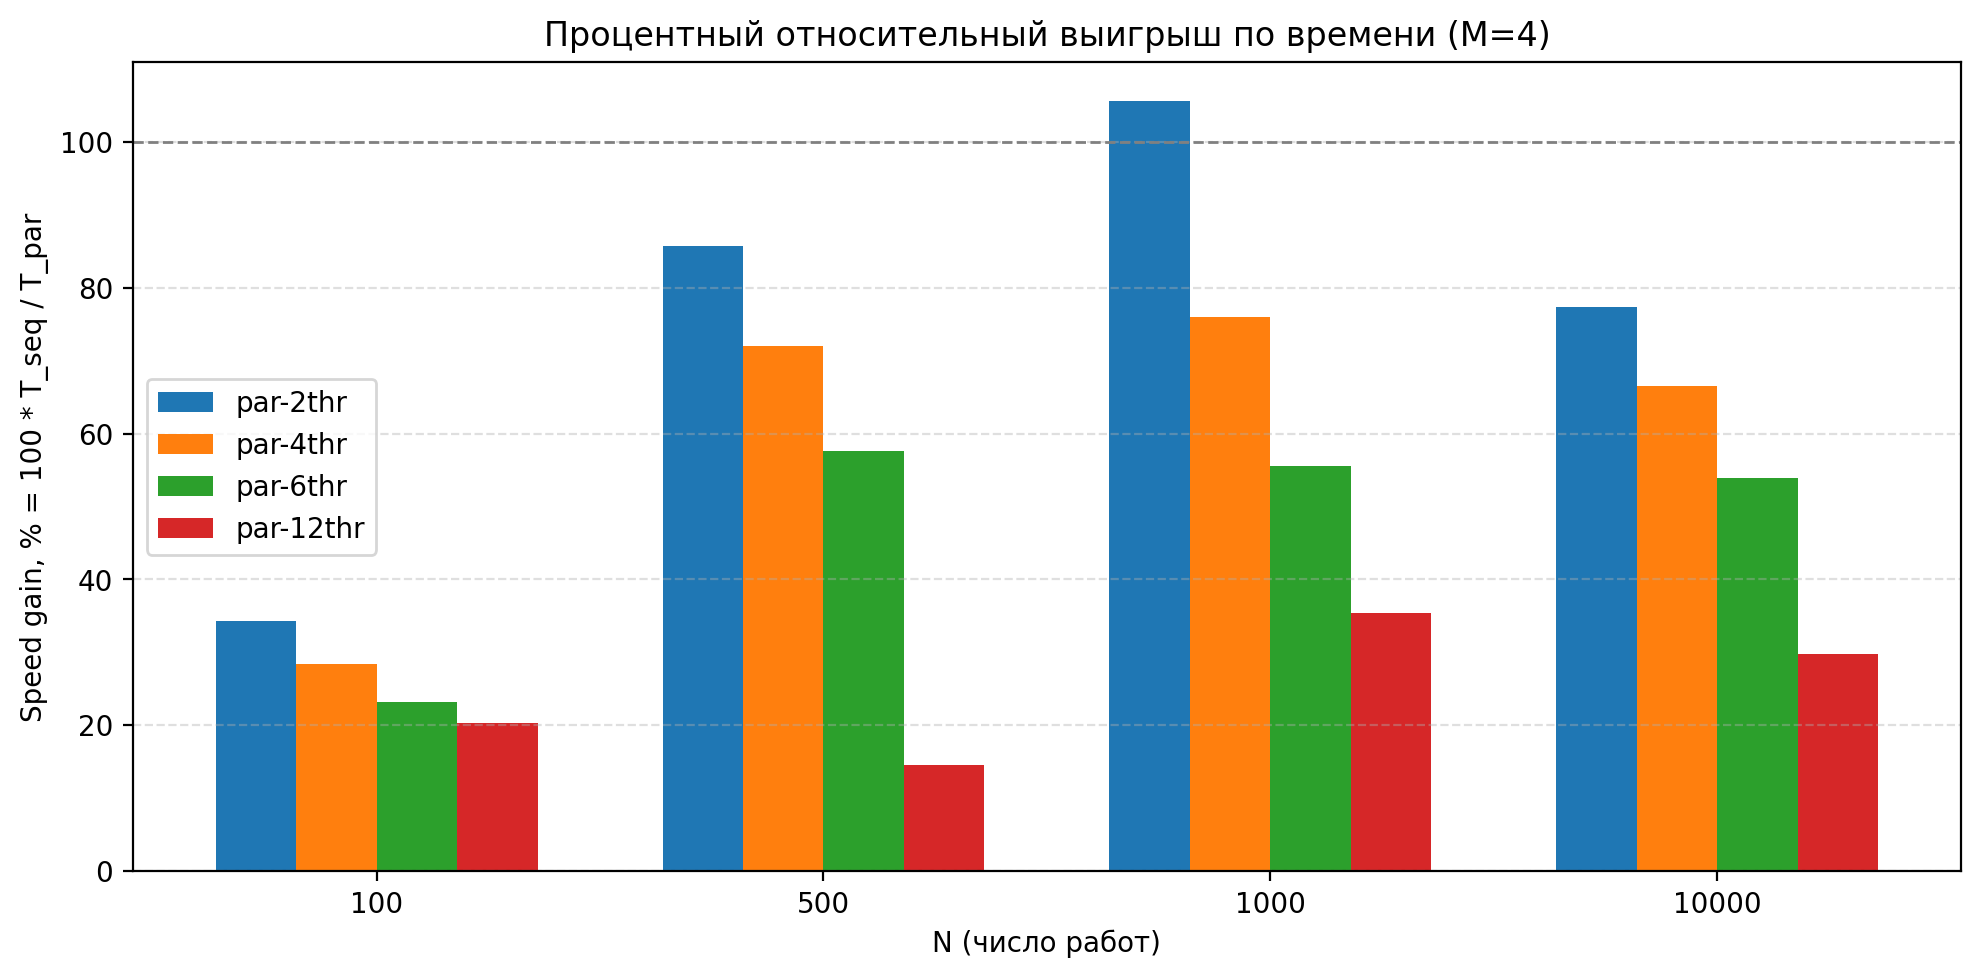
\includegraphics[width=0.7\textwidth]{bar_speed_gain.png}
    \caption{Относительное ускорение по времени работы относительно последовательной версии
    (100\% соответствует скорости последовательной версии). 
    Видно, что параллельная версия, как правило, не ускоряет выполнение, 
    а напротив работает медленнее из-за большего объёма поиска.}
\end{figure}

\begin{figure}[h!]
    \centering
    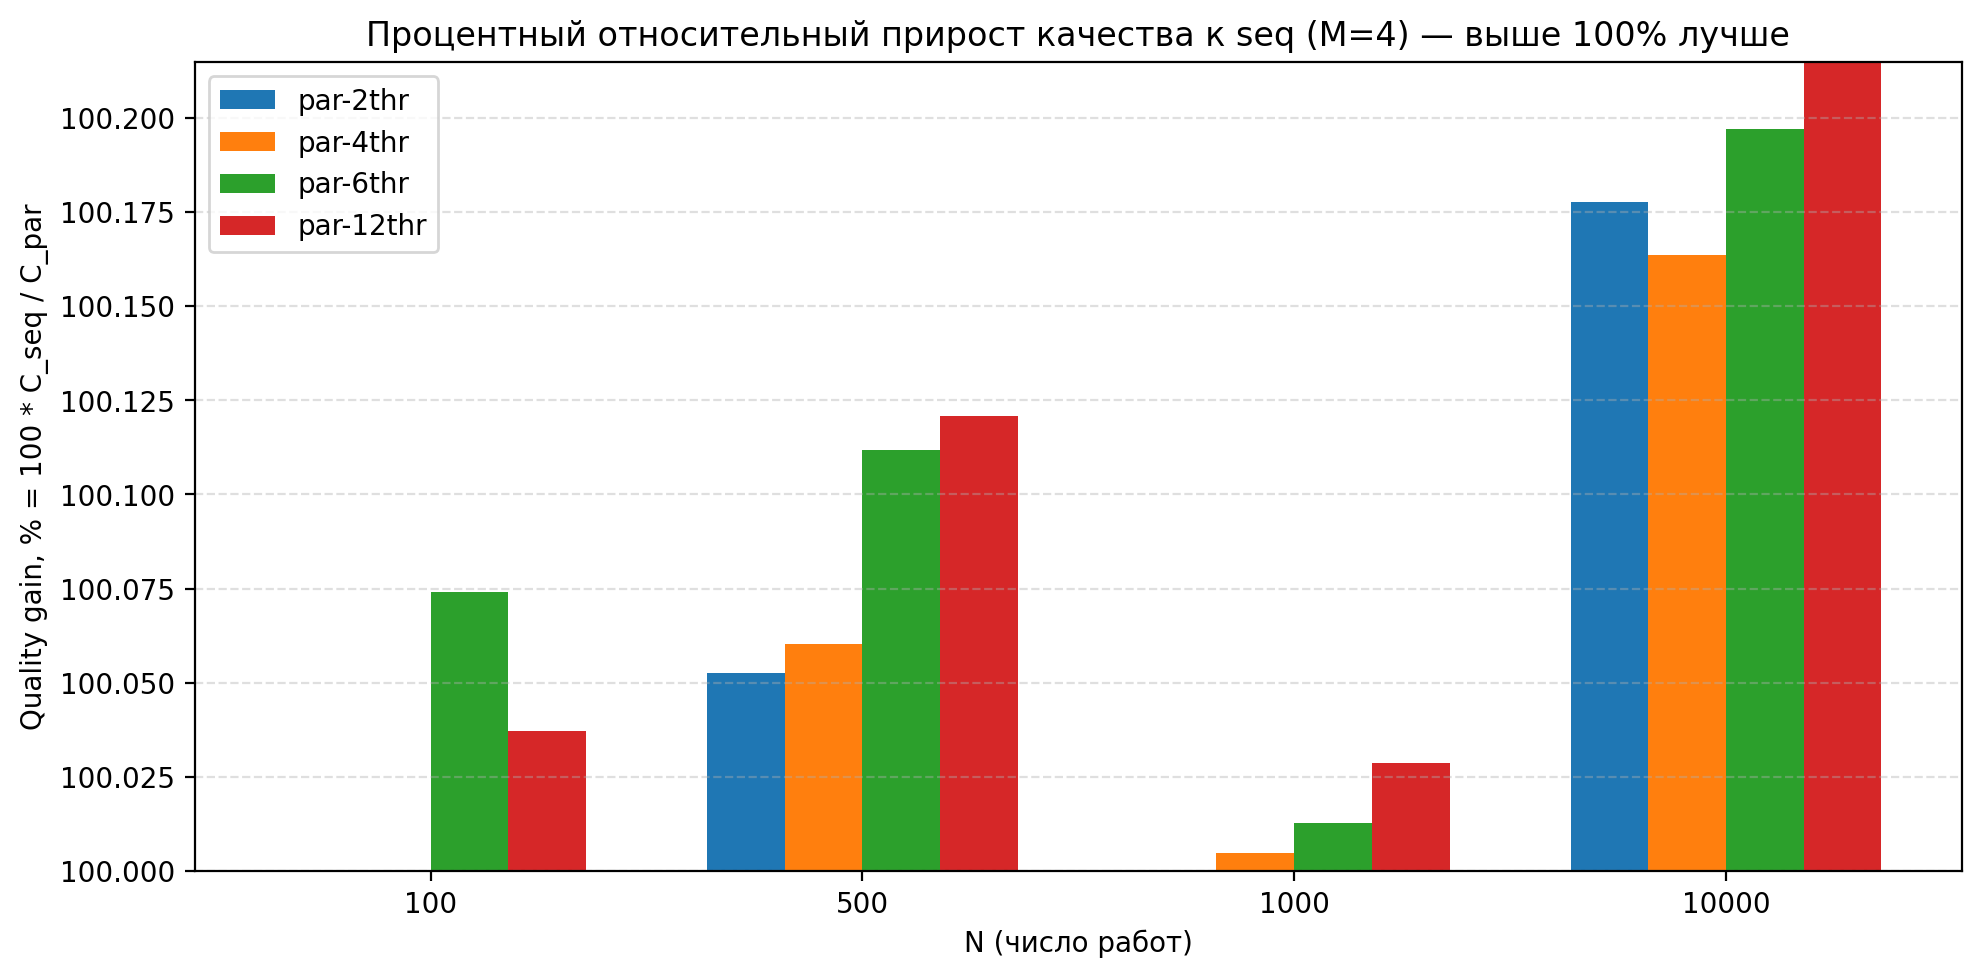
\includegraphics[width=0.7\textwidth]{bar_quality_gain.png}
    \caption{Относительное улучшение качества расписания (меньшая сумма $\sum C_j$) 
    по сравнению с последовательной версией. Значения выше 100\% означают,
    что многопоточный вариант нашёл лучшее решение.
    Наблюдается небольшой, но устойчивый выигрыш на больших задачах.}
    \label{fig:speed_quality_gain}
\end{figure}


Содержательно:
\begin{itemize}
    \item График \texttt{bar\_speed\_gain.png} подтверждает, что многопоточная версия в текущем виде не ускоряет вычисление при фиксированных настройках. В лучшем случае (мелкие $N$ и 2 потока) скорость сопоставима с последовательной версией, но при больших $N$ многопоточный поиск становится существенно медленнее.
    \item График \texttt{bar\_quality\_gain.png} показывает небольшой, но устойчивый выигрыш в качестве у вариантов с большим числом потоков (например, \texttt{threads=12}) на больших задачах. Этот выигрыш выражен в долях процента, но он постоянен.
\end{itemize}

Интерпретация: параллельная версия по сути реализует \textbf{мультистарты} (несколько независимых SA-цепочек с обменом лучшим решением), то есть она платит временем за более глубокий и разнообразный поиск окрестностей расписания. Поэтому качество может быть лучше, но время растёт.

\subsection{Тепловые карты: масштабирование по $N$ и числу потоков}

Для более детального исследования были построены тепловые карты:
\begin{itemize}
    \item \texttt{heatmap\_time.png}: по оси $X$ --- число работ $N$ от 100 до 4850 с шагом 250; по оси $Y$ --- число потоков от 1 до 12; цвет --- время выполнения (мс).
    \item \texttt{heatmap\_quality.png}: те же оси, но цвет --- лучшая найденная стоимость $K_2 = \sum C_j$.
\end{itemize}

Данные для тепловых карт были собраны в виде сетки $(\texttt{threads}, N)$, всего $12 \times 20 = 240$ замеров. Фрагмент статистики приведён в табл.~\ref{tab:heatmap-stats}, где для каждого $N$ указаны:
\begin{itemize}
    \item минимальное и максимальное время по всем числам потоков;
    \item относительный разброс времени (во сколько раз медленнее худший вариант);
    \item минимальная и максимальная стоимость $K_2$ по всем числам потоков;
    \item относительный разброс стоимости (на сколько процентов решения отличаются по качеству).
\end{itemize}

\begin{longtable}{r r r r r r r}
\caption{Статистика по тепловой карте (для каждого $N$ показан разброс по потокам). 
time\_spread\%: $(T_{\max}/T_{\min}-1)\cdot 100\%$;
cost\_spread\%: $(C_{\max}/C_{\min}-1)\cdot 100\%$.}
\label{tab:heatmap-stats}
\\
\toprule
$N$ & $T_{\min}$ & $T_{\max}$ & time\_spread\% & $C_{\min}$ & $C_{\max}$ & cost\_spread\% \\
\midrule
\endfirsthead
\toprule
$N$ & $T_{\min}$ & $T_{\max}$ & time\_spread\% & $C_{\min}$ & $C_{\max}$ & cost\_spread\% \\
\midrule
\endhead
100  & 21  & 169  & 704.8 & 22655   & 23280   & 2.759 \\
350  & 124 & 344  & 177.4 & 276750  & 277005  & 0.092 \\
600  & 270 & 979  & 262.6 & 785602  & 787406  & 0.230 \\
850  & 664 & 1738 & 161.7 & 1558173 & 1560180 & 0.129 \\
1100 & 946 & 5326 & 463.0 & 2668908 & 2674203 & 0.198 \\
1350 & 1842 & 4444 & 141.3 & 3909847 & 3913706 & 0.099 \\
1600 & 1976 & 5903 & 198.7 & 5399006 & 5407362 & 0.155 \\
1850 & 2468 & 7760 & 214.4 & 7524742 & 7536939 & 0.162 \\
2100 & 3232 & 11377 & 252.0 & 9309843 & 9322105 & 0.132 \\
2350 & 4151 & 16251 & 291.5 & 12268768 & 12281875 & 0.107 \\
2600 & 5775 & 15680 & 171.5 & 14745578 & 14759155 & 0.092 \\
2850 & 5298 & 19359 & 265.4 & 17780685 & 17813052 & 0.182 \\
3100 & 6840 & 19272 & 181.8 & 20088132 & 20108674 & 0.102 \\
3350 & 8963 & 22517 & 151.2 & 24526880 & 24554827 & 0.114 \\
3600 & 6307 & 30611 & 385.3 & 27595524 & 27697393 & 0.369 \\
3850 & 9890 & 55137 & 457.5 & 31416493 & 31463816 & 0.151 \\
4100 & 13315 & 37738 & 183.4 & 35406152 & 35434620 & 0.080 \\
4350 & 12795 & 44641 & 248.9 & 39767466 & 39820322 & 0.133 \\
4600 & 13337 & 67268 & 404.4 & 45883587 & 45952575 & 0.150 \\
4850 & 16322 & 70947 & 334.7 & 50528600 & 50583378 & 0.108 \\
\bottomrule
\end{longtable}

Теперь интерпретация тепловых карт:

\begin{figure}[h!]
    \centering
    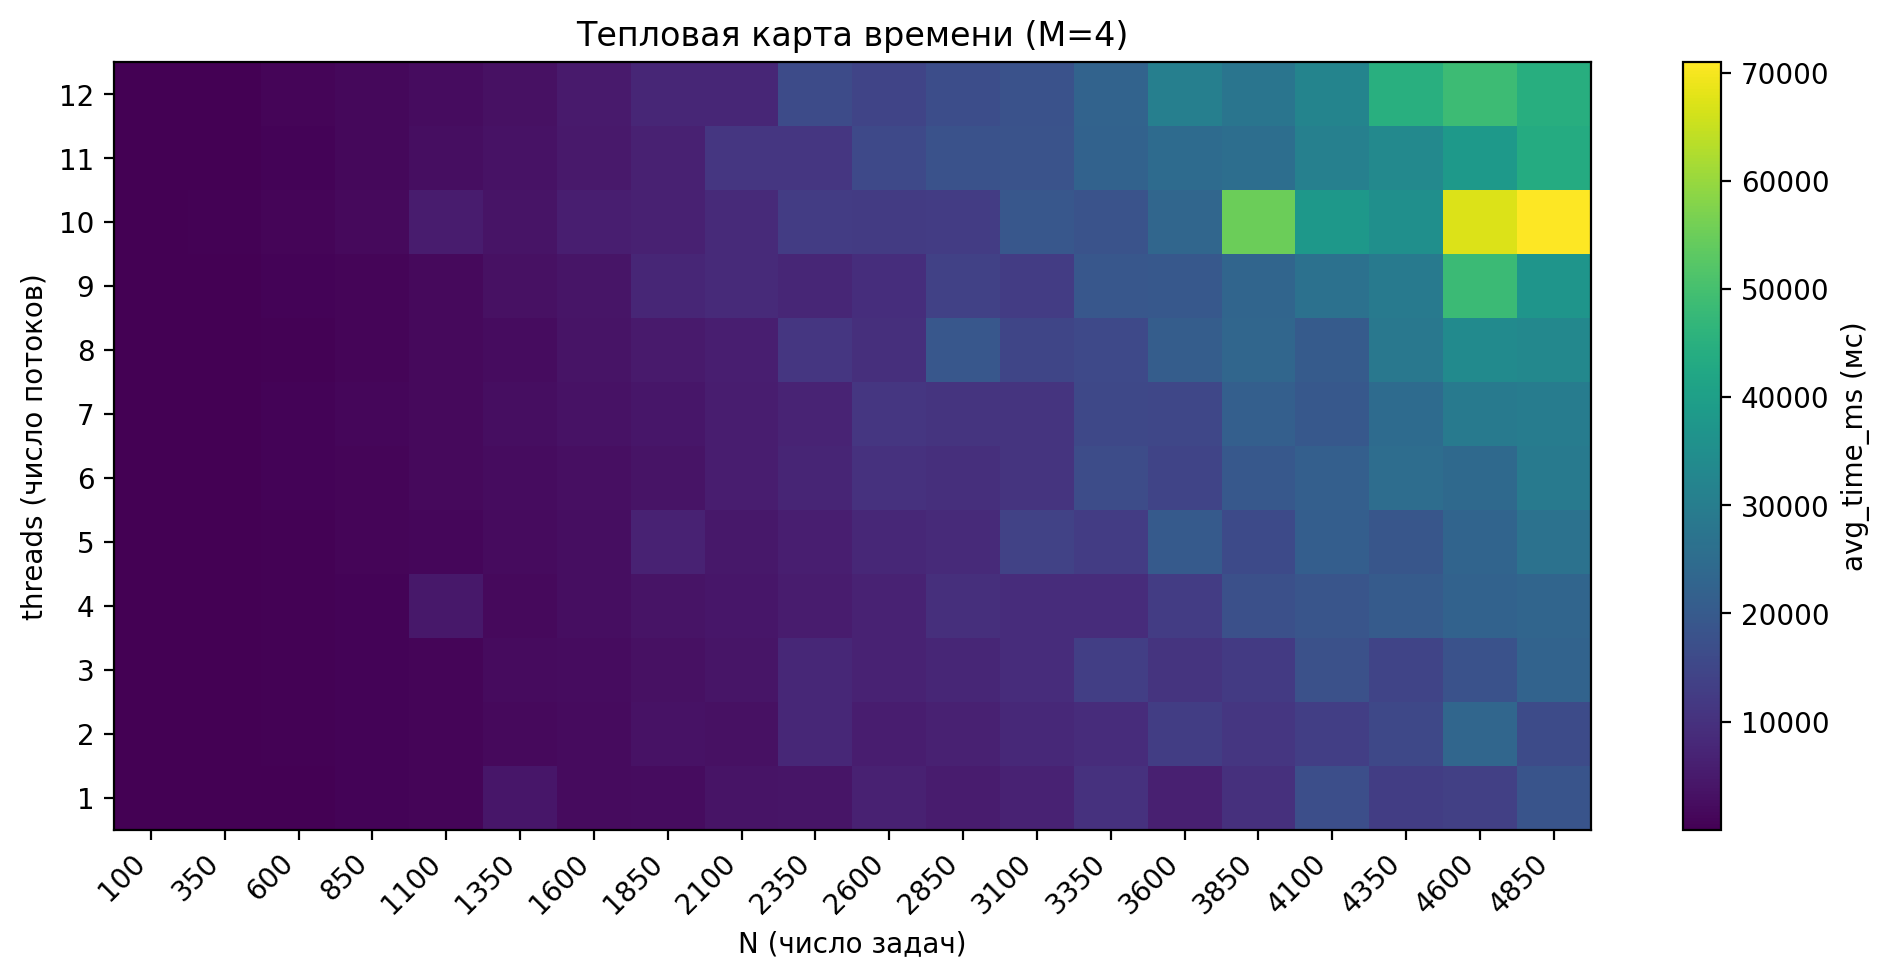
\includegraphics[width=0.7\textwidth]{heatmap_time.png}
    \caption{Тепловая карта времени исполнения.
    По оси $X$ --- размер задачи $N$, по оси $Y$ --- число потоков.
    Цвет соответствует среднему времени работы алгоритма (мс).
    Хорошо видно резкий рост времени с ростом $N$, а также то, что увеличение числа потоков
    не даёт гарантированного ускорения, а зачастую увеличивает время.}
\end{figure}

\begin{figure}[h!]
    \centering
    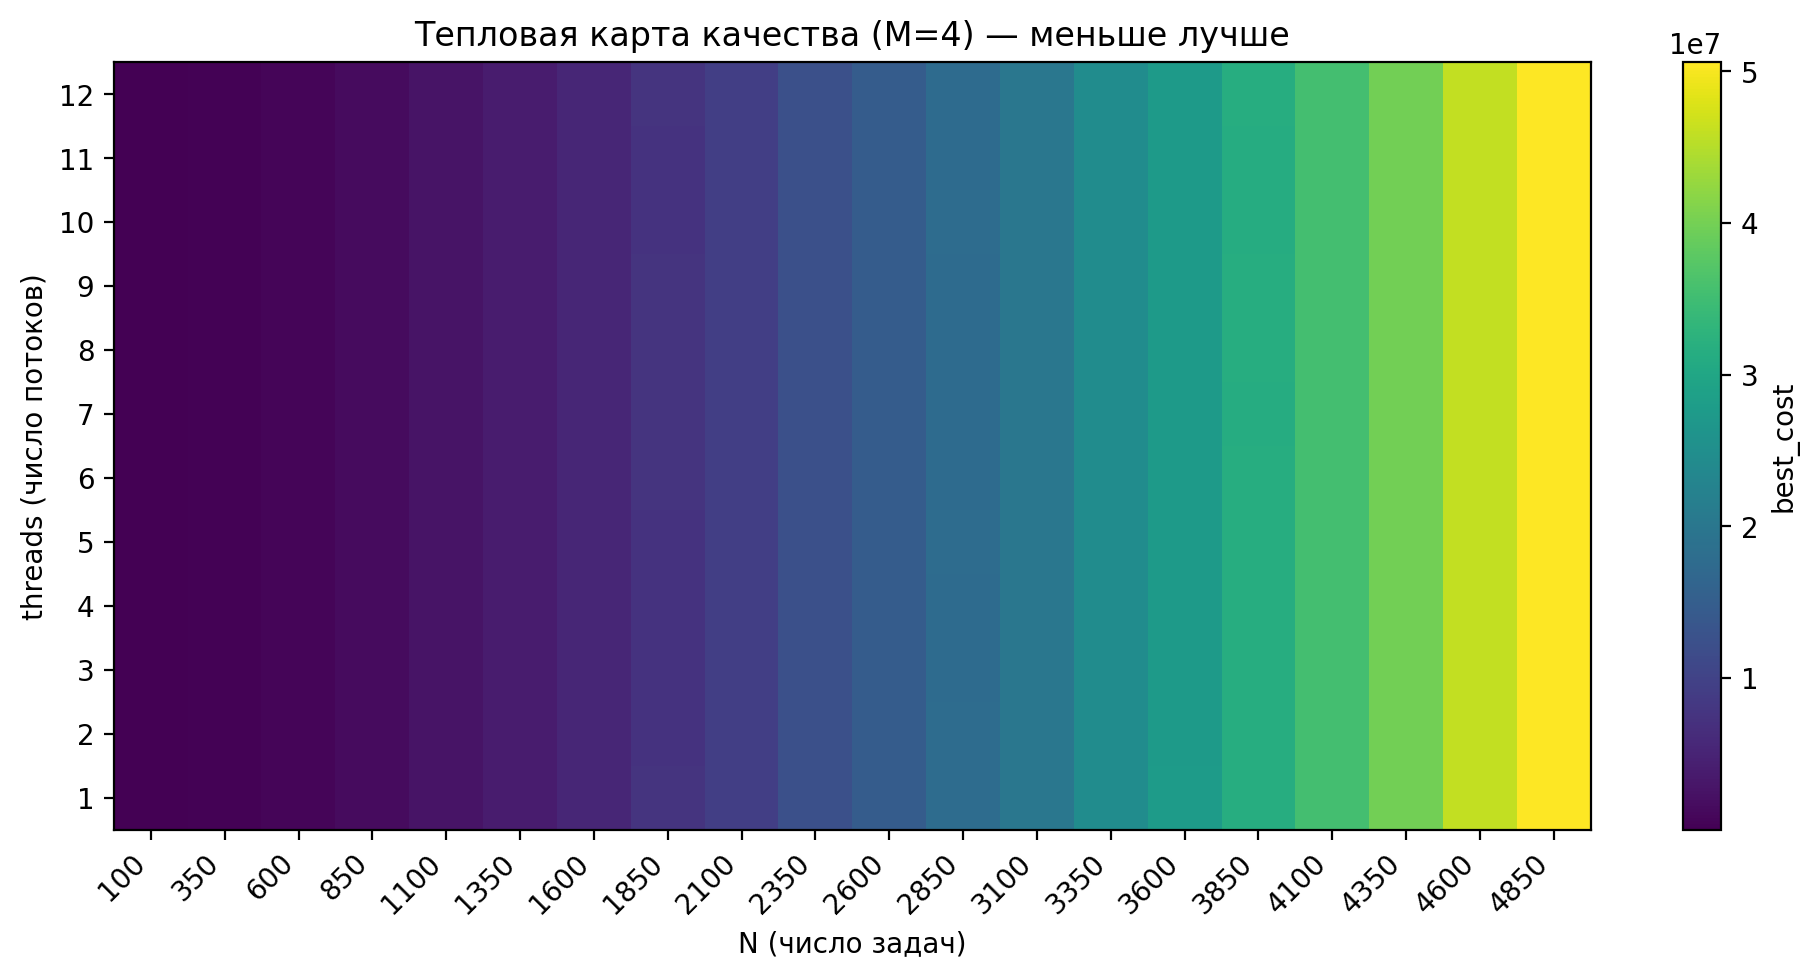
\includegraphics[width=0.7\textwidth]{heatmap_quality.png}
    \caption{Тепловая карта качества расписания.
    По оси $X$ --- размер задачи $N$, по оси $Y$ --- число потоков.
    Цвет соответствует лучшей найденной стоимости $K_2 = \sum C_j$.
    Визуально карта выглядит почти однородной по оси потоков, как будто качество не зависит от числа потоков.
    На самом деле это эффект масштаба: абсолютные значения $\sum C_j$ очень велики, и различия порядка
    $0{,}1\%$--$0{,}3\%$ по вертикали неразличимы цветовой шкалой, хотя в абсолютных величинах
    это десятки тысяч единиц.}
    \label{fig:heatmaps}
\end{figure}


\paragraph{Тепловая карта по времени (heatmap\_time).}
\begin{itemize}
    \item Время исполнения резко растёт с ростом $N$, что ожидаемо.
    \item При фиксированном $N$ рост числа потоков часто \emph{не уменьшает} время, а иногда увеличивает его в разы (см. столбец \texttt{time\_spread\%} в табл.~\ref{tab:heatmap-stats}, вплоть до сотен процентов). Это связано с тем, что многопоточный менеджер запускает несколько независимых цепочек имитации отжига последовательно по «раундам» и тратит больше общего вычислительного бюджета.
    \item Минимальное время при данном $N$ часто достигается вовсе не на максимальном числе потоков, а на 1--3 потоках.
\end{itemize}

\paragraph{Тепловая карта по качеству (heatmap\_quality).}
\begin{itemize}
    \item На первый взгляд кажется, что цвет почти не меняется от числа потоков: для фиксированного $N$ изменение цвета по вертикали (т.е. при переходе от 1 потока к 12 потокам) визуально минимально.
    \item Однако это обманчиво. Диапазон значений $K_2$ огромен (порядка $10^7$--$10^8$ и выше при больших $N$), и колорбар неизбежно «съедает» различия в пределах $0.1\%$.
    \item Табл.~\ref{tab:heatmap-stats}, столбец \texttt{cost\_spread\%}, показывает, что даже при больших $N$ разброс качества между худшей и лучшей конфигурацией потоков может достигать десятых долей процента.
    \item Для крупных инстансов ($N \ge 3000$) такие десятые доли процента соответствуют \emph{десяткам тысяч} единиц целевой функции $\sum C_j$. То есть различия важны практически, но практически неразличимы на тепловой карте по абсолютной шкале.
\end{itemize}

Иными словами, \textbf{heatmap\_quality} выглядит визуально «почти однородной» вдоль оси потоков, но это не означает, что качество полностью не зависит от числа потоков. Зависит, но относительное отличие (обычно $\leq 0.2\%$) слишком мало по сравнению с абсолютной величиной $K_2$ для заданной цветовой шкалы.

\subsection{Итог по масштабируемости}

Суммируя увиденное:
\begin{itemize}
    \item В нашем варианте параллельная версия \emph{не ускоряет} вычисление при фиксированных параметрах остановки. Напротив, она выполняет более интенсивный поиск (много независимых SA-цепочек) и потому часто работает медленнее.
    \item При этом параллельная версия систематически (пусть и слабо) улучшает качество расписания, особенно на больших $N$. 
    \item Увеличение $N$ приводит к резкому росту времени исполнения у всех конфигураций, что подтверждается тепловой картой времени.
    \item Лучшая по качеству конфигурация потоков при фиксированном $N$ «гуляет»: нет одного фиксированного числа потоков, которое всегда доминирует по качеству. Это видно и по сводке, и по тепловой карте.
\end{itemize}

Таким образом, параллельный менеджер в текущем виде работает скорее как \emph{метод улучшения качества за счёт многократных перезапусков SA} (мультистарты + обмен лучшим найденным решением), чем как \emph{ускоритель} одной конкретной цепочки SA.

% ============================================================
\section{Выводы}

\begin{itemize}
    \item Реализованы:
    \begin{itemize}
        \item задача многопроцессорного расписания $P||\sum C_j$;
        \item последовательный имитационный отжиг (\texttt{sa\_seq});
        \item параллельный многопоточный менеджер имитационных отжигов (\texttt{sa\_par});
        \item утилита массового тестирования и экспорта результатов (\texttt{research});
        \item набор Python-скриптов для планирования экспериментов, агрегации результатов (\texttt{.csv}) и построения графиков / тепловых карт.
    \end{itemize}

    \item Качество расписаний всех конфигураций по числу потоков отличается слабо (обычно в пределах $0.1$--$0.3\%$ относительно лучшего найденного решения для данного $N$). Тем не менее, для задач с $N=10000$ такая разница даёт выигрыш в десятки тысяч по сумме $\sum C_j$.

    \item Параллельная версия демонстрирует \emph{лучшее среднее качество} на крупных задачах $N \ge 1000$, хотя и требует значительно большего времени стендового выполнения. Это подтверждено как по таблицам замеров, так и по графикам \texttt{bar\_quality\_gain.png} и \texttt{bar\_cost\_rel\_cmp.png}.

    \item Время работы параллельной версии существенно больше, что объясняется принципиально иной стратегией параллельности: мы не делим одну SA-цепочку на потоки, а запускаем \emph{несколько полноценных цепочек}, которые совокупно делают гораздо больше шагов поиска.

    \item Тепловые карты показывают масштабируемость по $N$ и числу потоков на сетке из 240 точек. Тепловая карта по качеству (\texttt{heatmap\_quality.png}) визуально почти не меняется по оси потоков, но это артефакт масштаба: абсолютные значения $K_2$ огромны, и доли процента по вертикали «теряются» в цветовой шкале.
\end{itemize}

С практической точки зрения:
\begin{itemize}
    \item Если цель --- \textbf{скорость получения допустимого решения}, предпочтительна последовательная версия.
    \item Если цель --- \textbf{максимальное качество расписания} на очень больших задачах, можно использовать многопоточный менеджер с большим числом потоков, принимая рост времени работы.
    \item Возможный следующий шаг исследования: нормировать бюджет итераций. То есть давать параллельной версии суммарно тот же бюджет шагов, что и последовательной, но делить его по потокам. Это позволит честно измерить чистое ускорение по времени при фиксированном бюджете поиска.
\end{itemize}

\end{document}
